\begin{figure*}[htbp]
\centering
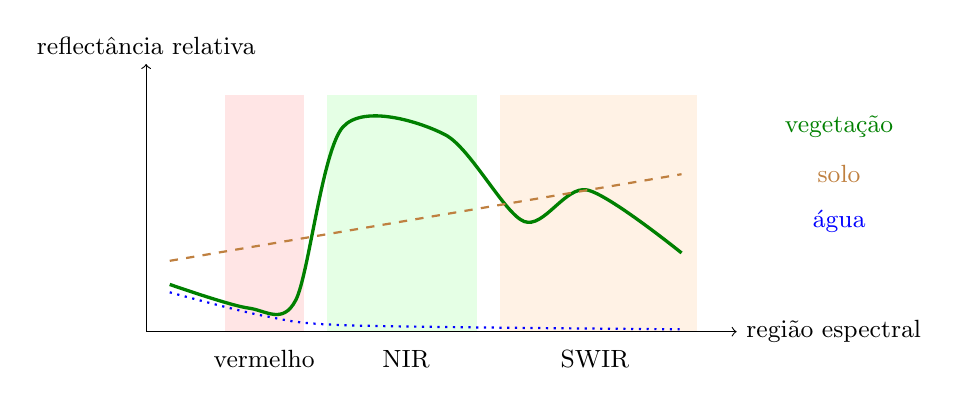
\begin{tikzpicture}[x=1cm,y=1cm,font=\small]
\fill[red!10] (1,0) rectangle (2,3);
\fill[green!10] (2.3,0) rectangle (4.2,3);
\fill[orange!10] (4.5,0) rectangle (7,3);
\draw[->] (0,0)--(7.5,0) node[right]{região espectral};
\draw[->] (0,0)--(0,3.4) node[above]{reflectância relativa};
\draw[very thick,green!50!black] plot[smooth] coordinates {(0.3,0.6)(1.3,0.3)(1.9,0.4)(2.5,2.6)(3.8,2.5)(4.8,1.4)(5.6,1.8)(6.8,1)};
\draw[thick,brown,dashed] (0.3,0.9)--(6.8,2);
\draw[thick,blue,dotted] plot[smooth] coordinates {(0.3,0.5)(1.5,0.2)(2.6,0.08)(6.8,0.03)};
\node at (1.5,-0.35){vermelho}; \node at (3.3,-0.35){NIR}; \node at (5.7,-0.35){SWIR};
\node[green!50!black] at (8.8,2.6){vegetação};
\node[brown] at (8.8,2){solo}; \node[blue] at (8.8,1.4){água};
\end{tikzpicture}
\caption{Comportamento espectral esquemático. Curvas qualitativas sem escala numérica, não medições. Fonte: elaborado pelo autor, síntese conceitual de \citet{WEISS2020}.}
\label{fig:espectro}
\end{figure*}
\begin{figure*}[htbp]
\centering\small
\begin{tabular}{lllll}
\hline Banda & Região & Centro S2A / S2B (nm) & Resolução & Índice no sistema\\ \hline
B4 & Vermelho & 664,5 / 665 & 10 m & NDVI\\
B8 & NIR amplo & 835,1 / 833 & 10 m & NDVI, NDWI\\
B8A & NIR estreito & 864,8 / 864 & 20 m & NDMI\\
B11 & SWIR & 1613,7 / 1610,4 & 20 m & NDWI, NDMI\\ \hline
\end{tabular}

\begin{tikzpicture}[x=0.009cm,y=0.6cm,font=\small]
\draw[->] (600,0)--(1730,0) node[right]{nm};
\foreach \x in {665,835,865,1614}{\draw[thick] (\x,0)--(\x,1);}
\node at (665,1.5){B4}; \node at (805,1.5){B8};
\node at (895,2){B8A}; \node at (1614,1.5){B11};
\end{tikzpicture}
\caption{Bandas dos índices. Centros espectrais por instrumento e resoluções nativas conforme o catálogo harmonizado \citep{GOOGLE_S2_SR}. Fonte: elaborado pelo autor.}
\label{fig:bandas}
\end{figure*}
\begin{figure*}[htbp]
\centering
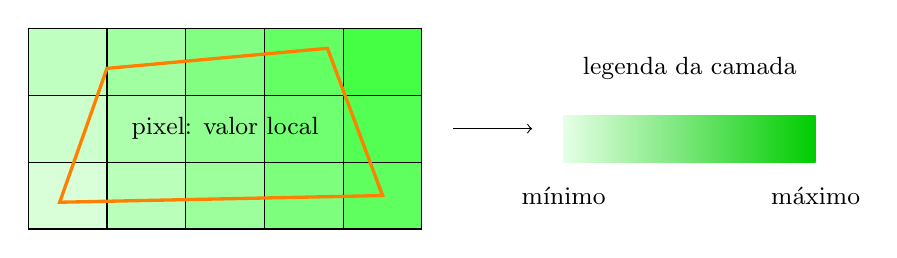
\begin{tikzpicture}[x=1cm,y=0.85cm,font=\small]
\foreach \x in {0,...,4}{\foreach \y in {0,...,2}{
\pgfmathtruncatemacro{\shade}{15+12*\x+5*\y}
\fill[green!\shade] (\x,\y) rectangle +(1,1);}}
\draw[step=1] (0,0) grid (5,3);
\draw[very thick,orange] (0.4,0.4)--(4.5,0.5)--(3.8,2.7)--(1,2.4)--cycle;
\node at (2.5,1.5){pixel: valor local};
\draw[->] (5.4,1.5)--(6.4,1.5);
\shade[left color=green!10,right color=green!80!black] (6.8,1) rectangle (10,1.7);
\node at (6.8,0.5){mínimo}; \node at (10,0.5){máximo};
\node at (8.4,2.4){legenda da camada};
\end{tikzpicture}
\caption{Polígono vetorial, células raster e gradiente em esquema sem dados reais. A geometria e as máscaras determinam o suporte válido. Fonte: elaborado pelo autor.}
\label{fig:raster-vetor}
\end{figure*}
\begin{figure*}[htbp]
\centering\small
\begin{tabular}{lcccl}
\hline & Pixel A & Pixel B & Média espacial & Operação\\ \hline
Aquisição 1 & 0,1 & 0,9 & 0,5 & média dos pixels\\
Aquisição 2 & 0,2 & 0,8 & 0,5 & média dos pixels\\
Aquisição 3 & 0,9 & 0,7 & 0,8 & média dos pixels\\ \hline
Mediana por pixel & 0,2 & 0,8 & 0,5 & média da composição\\ \hline
\end{tabular}
\caption{Ilustração matemática: a média das médias por aquisição é 0,6, enquanto a média da composição mediana é 0,5. Pesos iguais, sem máscaras; não é resultado experimental. Fonte: elaborado pelo autor.}
\label{fig:composicao}
\end{figure*}
\begin{figure*}[htbp]
\centering
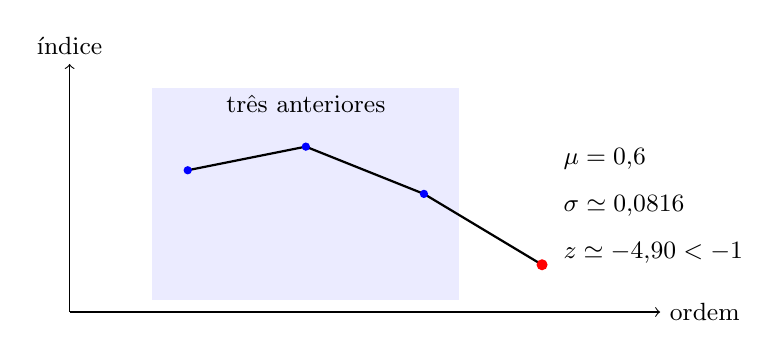
\begin{tikzpicture}[x=1.5cm,y=3cm,font=\small]
\fill[blue!8] (0.7,0.05) rectangle (3.3,0.95);
\draw[->] (0,0)--(5,0) node[right]{ordem};
\draw[->] (0,0)--(0,1.05) node[above]{índice};
\draw[thick] (1,0.6)--(2,0.7)--(3,0.5)--(4,0.2);
\foreach \x/\y in {1/0.6,2/0.7,3/0.5}{\fill[blue] (\x,\y) circle (1.5pt);}
\fill[red] (4,0.2) circle (2pt);
\node at (2,0.88){três anteriores};
\node[anchor=west] at (4.1,0.65){$\mu=0{,}6$};
\node[anchor=west] at (4.1,0.45){$\sigma\simeq0{,}0816$};
\node[anchor=west] at (4.1,0.25){$z\simeq-4{,}90<-1$};
\end{tikzpicture}
\caption{Janela e sinalização em sequência didática. Valores criados para ilustrar a regra, não observações agrícolas ou medida de eficácia. Fonte: elaborado pelo autor.}
\label{fig:janela}
\end{figure*}
